\subsection{Determination of $L$ and $C$}
The diameters of the inner and outer cylinders were measured using a manual micrometer five times and averaged to remove random errors. The mean values for the inner cylinder diameter, $a$, and outer cylinder diameter, $b$, are;
\[ a = 0.59 \pm 0.01 \ \text{mm}, \quad\quad b = 4.83 \pm 0.18 \ \text{mm} \]
with uncertainty values as the standard deviation. For the larger cylinder, the volume is far more malleable than the inner cylinder, which introduces greater error than the inner cylinder -- as when the micrometer is tightened, it can compress the material slightly -- adding a bias below the true diameter. \\ 

From Equations \ref{inductance} and \ref{conductance}, we can compute the inductance and conductance per unit length up to a scale factor from the dielectric material used in the wire.
\begin{align*}
    L &= \frac{ \ln \left( b \middle/ a \right) }{2 \pi \epsilon_o \epsilon_r c^2} = (0.334 \pm 0.013)\mu_0\mu_r \ \text{H m$^{-1}$} \\
    C &= \frac{2 \pi \epsilon_0\epsilon_0}{\ln \left( b \middle/ a \right) } = \frac{\epsilon_0\epsilon_r}{0.334 \pm 0.013} \ \text{F m$^{-1}$} 
\end{align*}
where $\epsilon_0 = 8.85\e{-12} $ Fm$^{-1}$ is the permittivity of free space, $\mu_0 = 1.2566\e{-6}$ Hm$^{-1}$ is the permeability of free space, $\epsilon_r$ is the relative permittivity of the dielectric separating the coaxial cylinders, and $\mu_r$ is the relative permeability of the dielectric (which we assume is approximately $\mu_r=1$ for future calculations).\\

\subsection{RF Input}

The acquired data points for both the open and short-circuited setups were fit using a custom function to determine the parameters. From Equation \ref{Zin_open} and \ref{Zin_short} and that we are examining only positive values we can define the fitting function to be,
\begin{align}
    |Z_\text{in}| &= A | \tan\left( B(f + C) \right)| + D f 
\end{align}

Where $A,B,C,D$ are the fitting coefficients and their respective units are determined through dimensional analysis. The linear term $Df$ is added to account for an experimental drift of increasing impedance at the resonance frequencies. This drift could be explained from attenuation of the signal through the wire.\\

\begin{table}[H]
    \centering
    \begin{tabular}{c|c|c}
        \textbf{Fit Coefficient} &  \textbf{Open Termination} & \textbf{Shorted Termination} \\ \midrule
        A & 46.03 $\pm$ 2.01 \ $\Omega$ & 43.5 $\pm$ 6.06 \ $\Omega$\\
        B & 1.909 $\pm$ 0.010 \ MHz$^{-1}$ & 1.902 $\pm$ 0.011 \ MHz$^{-1}$ \\
        C & -2.440 $\pm$ 0.17 \ MHz & -1.606 $\pm$ 0.023 \ MHz \\
        D & 4.142 $\pm$ 0.268 \ $\Omega$ MHz$^{-1}$ & 4.040 $\pm$ 0.268 \ $\Omega$ MHz$^{-1}$
    \end{tabular}
    \caption{Best fit coefficients using least squares method with the associated error the 95\% confidence interval of the fitting function. Fitting was performed using a custom Matlab (Mathworks Ltd) script.}
    \label{CoefficientsTable}
\end{table}

\begin{figure}[H]
    \centering
    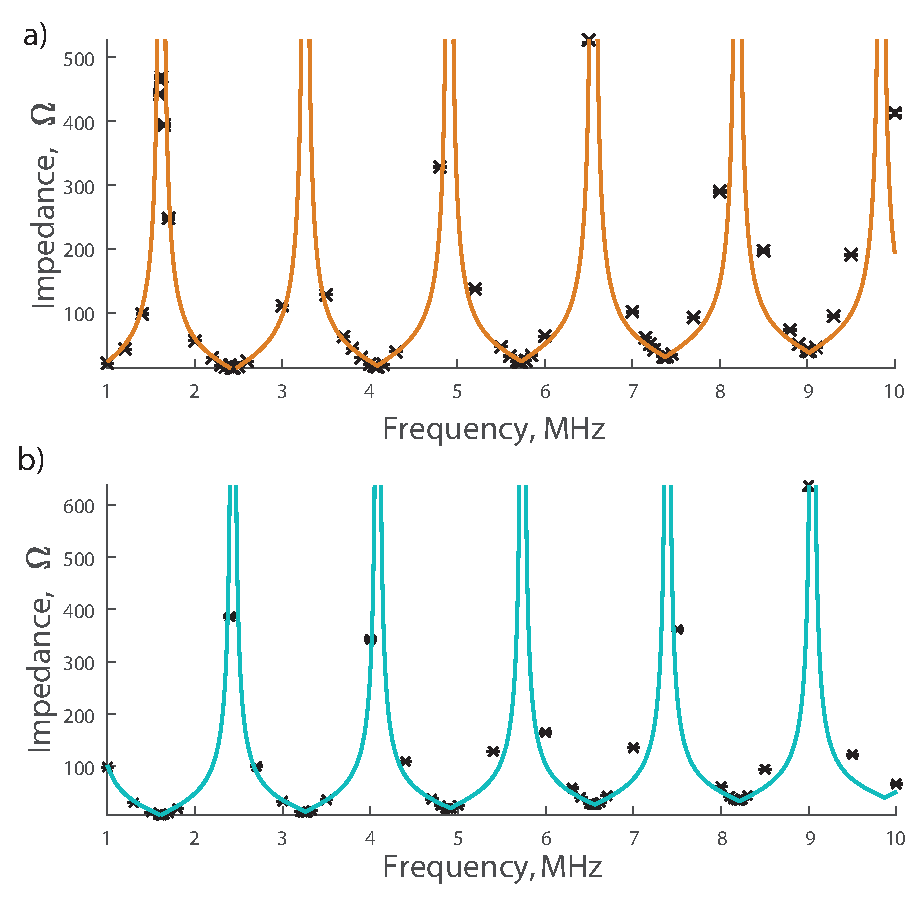
\includegraphics[width=\textwidth]{figures/Fit_V3.eps}
    \caption{Input impedance as function of the frequency. Crosses represent measured impedance values with corresponding y-error bars, while the solid lines are fit best fit via least squares method for \textbf{a)} open-ended circuit and \textbf{b)} short-circuited setup}
    \label{Zin_plot}
\end{figure}


The frequency difference between minimum impedance points is calculated from the fitting parameter $B$ as;
\begin{align}
    \Delta f_\text{open} &= \frac{\pi}{B_\text{open}} = 1.6457 \pm 0.0086  \ \text{MHz} \\
    \Delta f_\text{closed} &= \frac{\pi}{B_\text{closed}} = 1.6517 \pm 0.0087 \ \text{MHz}
\end{align}

The speed of the pulse can be computed with our calculation of the frequency spacing of the impedance minimums. With the knowledge that $v = \omega/k$ and assuming our impedance minimums are at $Z_\text{min} = 0$,

\begin{align}
    Z_\text{in} = 0 &= Z_0 |\tan(k x_\text{end})| \\
    &= \tan(k \ell) \\
    \arctan(0) &= k\ell \\
    n\pi &= \frac{\omega}{v} \ell\\
    n\pi &= \frac{2\pi f}{v} \ell\\
    v &= 2\Delta f \ell
\end{align}
With the length of the cable at $\ell = 60.0 \pm 0.1$ m and the frequency separation from above,

\begin{align} 
    & { v_\text{open} = (197.484 \pm 2.166 ) \times 10^{6} \ \text{ms$^{-1}$} } \label{open_vel} \\
    \intertext{This value is calculated using the measured frequency spacing for the open cable. A similar analysis is done for the measured values of shorted cable,}
    & { v_\text{closed} = (198.204 \pm 2.190 ) \e{6} \ \text{ms$^{-1}$} } \label{closed_vel} 
\end{align}

The average of these two values is considered the measurement of the velocity.
\begin{align}
    &\boxed{ v = (197.8440 \pm 1.5486) \e{6} \ \text{ms$^{-1}$} } \label{eqn:velocity}
\end{align}

With the measured values of $L$ and $C$, we can determine the dielectric used in the cables.
\begin{align}
    LC &= \left( \frac{k}{\omega}  \right)^2 = \frac{1}{v^2} \\
    \mu_0 \mu_r \epsilon_0 \epsilon_r &= \frac1{v^2} \\
    \shortintertext{Assuming that the relative permeability, $\mu_0$ is approximately 1,}
    \frac{\epsilon_r}{c^2} &= \frac1{v^2} \\
    \Rightarrow \epsilon_r &= \frac{c^2}{v^2}
\end{align}

So, the dielectric is computed with the velocity value from Equation \ref{eqn:velocity},
\begin{align}
    &\boxed{\epsilon_r = 2.2840 \pm 0.0358}
\end{align}
From a table of common dielectrics\cite{dielectric}, we conclude that this material is likely polyethelene, with a listed dielectric of $\epsilon_r = 2.26$. However, more tests would need to be done to cross-check results with.\\

Calculating our characteristic impedance with this value of the dielectric constant (assuming relative permeability is $\mu_r=1$),
\begin{align}
    Z_0 &= \sqrt{\frac{L}{C}} \\
    &= \sqrt{(0.334\pm0.013)^2\frac{\mu_0 \mu_r}{\epsilon_0 \epsilon_r}} \\
    &= 83.3 \pm 9.7 \ \Omega \label{eqn:characteristic_impedance}
\end{align}

We can also calculate the inductance and capacitance per unit length of the cable,
\begin{align}
    L &= (4.197 \pm 0.163)\e{-7} \ \text{H \ m}^{-1} \\
    C &= (6.055 \pm 0.236)\e{-11} \ \text{F\ m}^{-1}
\end{align}


\vspace{4mm}

The phase relationship near resonance and off-resonance between the current and the voltage waveforms for open, shorted, and matched cables are tabulated in Table \ref{tab:phase_relations}. This table summarizes which wave, either the current or voltage, is leading at frequencies just below, on, and just above resonance and off-resonance frequencies. We can see that for both the open and shorted cases, the leading wave switches at resonance and off-resonance frequencies -- but they are opposite between open and shorted. The leading wave also flips between the open and shorted case, as we expect based on the change in our boundary condition of the cable termination. For the matched termination, the phase shift between voltage and current is constant over frequency, with the voltage always slightly leading over the current.\\
\begin{table}[H]
    \centering
    \begin{tabular}{c||c|c||c|c}
         &  \multicolumn{2}{c}{\textbf{Minimum Impedance}} &  \multicolumn{2}{c}{\textbf{Maximum Impedance}} \\
        \textbf{Termination} & Frequency & Leading Wave & Frequency & Leading Wave \\ \midrule
        Open & $f \lesssim f_\text{min}$ & Current & $f \lesssim f_\text{max}$ & Voltage \\
        
        & $f=f_\text{min}$ & In-phase & $f=f_\text{max}$ & In-phase \\
        
        & $f\gtrsim f_\text{min}$ & Voltage & $f\gtrsim f_\text{max}$ & Current\\ \midrule
        
        Shorted & $f \lesssim f_\text{min}$ & Voltage & $f \lesssim f_\text{max}$ & Current \\
        & $f=f_\text{min}$ & In-phase & $f=f_\text{max}$ & In-phase \\
        & $f\gtrsim f_\text{min}$ & Current & $f\gtrsim f_\text{max}$ & Voltage \\ \midrule
        
        Matched & $f \lesssim f_\text{min}$ & Voltage & $f \lesssim f_\text{max}$ & Voltage \\
        & $f=f_\text{min}$ &Voltage & $f=f_\text{max}$ & Voltage \\
        & $f\gtrsim f_\text{min}$ & Voltage & $f\gtrsim f_\text{max}$ & Voltage \\ \midrule
    \end{tabular}
    \caption{Phase relations between voltage and current for open, shorted and matched cables. $f_\text{min}$ and $f_\text{max}$ are the frequency values at which the minimum and maximum impedance occur, respectively. The leading wave is either the current or voltage signal which has a positive phase shift relative to the other.}
    \label{tab:phase_relations}
\end{table}

Other analogous LCR circuits which give rise to such phase trends are \textbf{series resonance circuits} consisting of a single resistor, inductor, and capacitor wired in series with an AC power supply (see Figure \ref{fig:lrc_circuit}). If the components are in this series order, then below resonance the voltage leads, at resonance the voltage and current are in phase, and above resonance the current signal leads.\\

\begin{figure}[H]
    \centering
    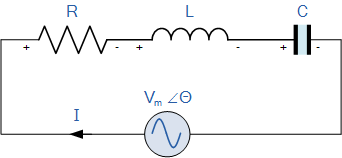
\includegraphics[width=0.5\textwidth]{figures/acp200.png}
    \caption{LCR circuit which provides similar phase trends between the voltage and current signals as a the coaxial cable demonstrates \cite{lrc}.}
    \label{fig:lrc_circuit}
\end{figure}

\vspace{5mm}

For the open termination case, there will be a current node at the ends (and thus an impedance maximum) and the resonant frequencies are given by,
\begin{align}
    \frac{2n+1}{2} \pi &= \frac{2\pi f \ell}{v} \\
    \intertext{And similarly for the closed termination case,}
    n\pi &= \frac{2\pi f \ell}{v}
\end{align}
These theoretical resonance frequencies are tabulated in Tables \ref{tab:open_resonance_freqs} and \ref{tab:closed_resonance_freqs}, and we can see that our expected values for the resonance frequencies match closely with the experimental data points from the custom fit in Figure \ref{Zin_plot}. The expected and measured resonant frequencies agree within one decimal place, but falling slightly outside the uncertainty bounds of the expected values.
\begin{table}[H]
    \centering
    \begin{tabular}{c|c|c|c}
        $n$ & $f(Z_\text{min})$, MHz &  $Z_\text{min}, \ \Omega$ & \textbf{Theoretical} $f(Z_\text{min})$, MHz \\
        2 & 2.4401 & 10.1169 & 2.4731 $\pm$ 0.0198\\
        3 & 4.0855 & 16.9295 & 4.1217 $\pm$ 0.0330\\
        4 & 5.7309 & 23.7636 & 5.7704 $\pm$ 0.0462\\
        5 & 7.3771 & 30.5845 & 7.4192 $\pm$ 0.0594\\
        6 & 9.0225 & 37.3794 & 9.0679 $\pm$ 0.0726\\
    \end{tabular}
    \caption{Open termination: Measured and expected resonance frequencies, along with corresponding experimental minimum impedance, for an open termination cable, 60 m long.}
    \label{tab:open_resonance_freqs}
\end{table}


\begin{table}[H]
    \centering
    \begin{tabular}{c|c|c|c}
          $n$ & $f(Z_\text{min})$, MHz &  $Z_\text{min}, \ \Omega$ & \textbf{Theoretical} $f(Z_\text{min})$, MHz \\
        1 & 1.6067 & 6.5128 & 1.6487 $\pm$0.0132  \\
        2 & 3.2583 & 13.1762 & 3.2974 $\pm$0.0264  \\
        3 & 4.9109 & 19.8662 & 4.9461 $\pm$ 0.0396 \\
        4 & 6.5626 & 26.5203 & 6.5948 $\pm$ 0.0528 \\
        5 & 8.2151 & 33.2196 & 8.2435 $\pm$ 0.0660 \\
        6 & 9.8668 & 39.8644 & 9.8922 $\pm$ 0.0792 \\
    \end{tabular}
    \caption{Shorted termination: Measured and expected resonance frequencies, along with corresponding experimental minimum impedance, for an shorted termination cable, 60 m long.}
    \label{tab:closed_resonance_freqs}
\end{table}


\subsection{Pulse Input}

\begin{figure}[H]
    \centering
    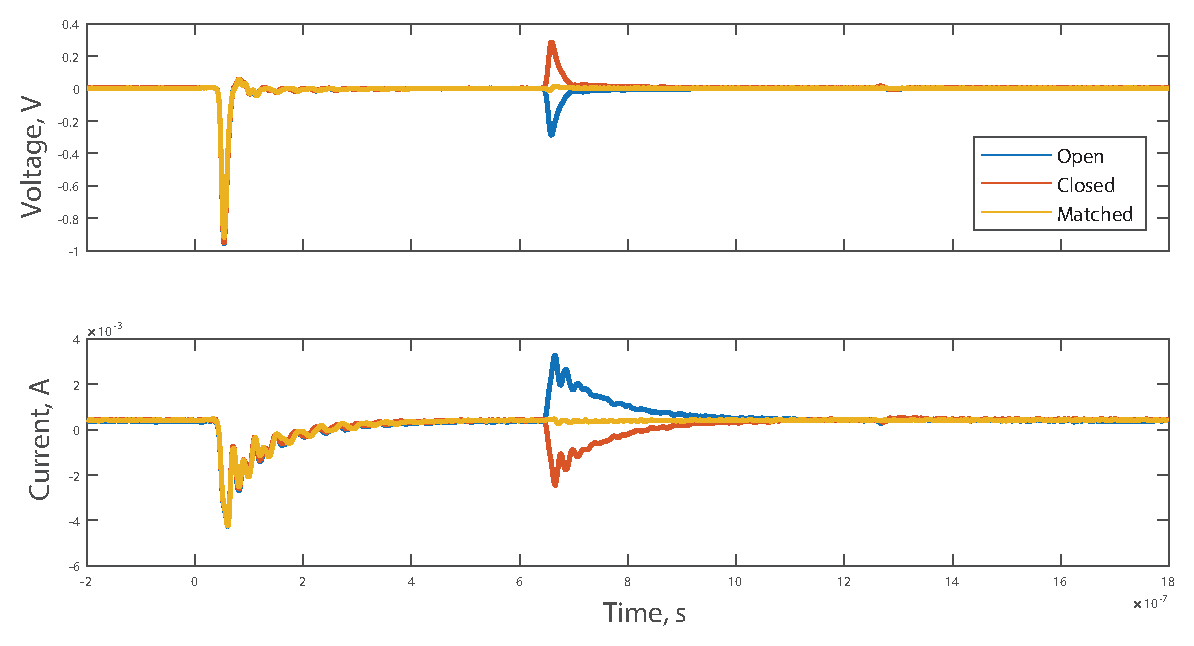
\includegraphics[width=\textwidth]{figures/TimePlot_V1.eps}
    \caption{Voltage and current traces over time for three termination cases (open, shorted, and matched) with single pulses as input. The secondary peaks are the reflected pulses returning after one round-trip of the coaxial cable.}
    \label{fig:time_plot}
\end{figure}
From Figure \ref{fig:time_plot} we see that for the open termination, the reflected current pulse is inverted as the there is a current node at $x=x_\text{end} = \ell$, while the voltage pulse is not inverted. Conversely, for shorted termination the opposite is true and the current is not inverted while voltage is. When the load is matched, we do not have a reflected pulse as the matched impedance mimics an infinitely long cable where no reflections can be produced.\\

The matched load resistance was measured at the point which minimized (removed) the reflection peak as viewed on an oscilloscope. The resistance uncertainty was determined through the measurement of the upper and lower bounds for where the reflected peak was still approximately zero to the naked eye.
\begin{align}
    Z_\text{matched} &= 76.4 \pm 2.0 \ \Omega
\end{align}
Comparing this to the value calculated in the earlier part, Equation \ref{eqn:characteristic_impedance}, we see that this value is in the error bounds of the first calculation -- but the uncertainty in this measurement is much lower as we have not propagated uncertainty through the calculation and this was a direct measurement. Thus, the value measured in this section, $Z_\text{matched} = 76.4 \pm 2.0 \ \Omega$ is better suited for future calculations.\\

The time delay between the first peak and second peak is $\Delta t = 60.4 \ \mu$s\footnote{The time resolution of the oscilloscope data is 2 ns, which we have omitted as it is negligible in the calculations. However, the uncertainty in the length of the cable is significant.}. The velocity is then,
\begin{align}
    v &= \frac{\Delta x}{\Delta t} = \frac{2\ell}{\Delta t}\\
    &= \frac{120.0 \pm 0.2}{60.4\times10^{-6}} \\
    &= (198.68 \pm 0.33) \times 10^{6} \ \text{ms$^{-1}$}
\end{align}

When we perform the same observation with 18 m and 9 m cables, the pulses are closer together in time, as expected. While no exact measurements were taken, the peaks are approximately 1/3 closer together in the 18 m cable case compared to the 60 m, and 1/6 closer for the 9 m cable -- as we expect to see. \\

When the buffer impedance is set to greater than the cable impedance, we see a pulse train caused by multiple reflections of the original pulse at each end of the cable. The amplitude of these peaks decrease as the buffer impedance increases, as there is more attenuation of the signal during each round trip through the cable. Similarly, when the buffer impedance is set to less than the cable impedance, we again observe a similar pulse train with each pulse separated by the time to travel the length of the cable and back. Conversely, with the buffer impedance lower that the characteristic impedance the amplitude of each pulse increases as the buffer impedance is lowered, as there is less attenuation of the signal.\\

To calculate the values of $L$ and $C$,
\begin{align}
    & Z_0 = \sqrt{\frac{L}{C}}, \quad & \left(\frac{k}{\omega}\right)^2 = \frac1{v^2} = LC 
\end{align} 
So, we can express the inductance and capacitance as,
\begin{align}
    Z_0 = \sqrt{L^2 v^2} = Lv \ \Rightarrow \ \boxed{L = \frac{Z_0}{v}} \\
    Z_0 = \sqrt{\frac1{C^2 v^2}} = \frac{1}{Cv} \ \Rightarrow \ 
    \boxed{C =\frac1{Z_0 v}} \\
\end{align}

So,
\begin{align}
    L &= \frac{Z_0}{v} = \frac{76.4 \pm 2.0}{(198.68 \pm 0.33) \e{6}} \\
    &= (4.5293 \pm 0.1189) \e{-7} \ \text{H\ m}^{-1}
\end{align}

Similarly,
\begin{align}
    C &= \frac1{Z_0 v} = \frac1{(76.4 \pm 2.0)(198.68 \pm 0.33) \e{6}} \\
    &= (7.7597 \pm 0.2037)\e{-11} \ \text{F\ m}^{-1}
\end{align}

